\section{Evaluation} \label{sec:eval}

\begin{table}[t]
\begin{center}
\begin{tabular}{|c|c|c|c|c|c|}\hline
& & \multicolumn{2}{|c|}{original} & \multicolumn{2}{|c|}{incremental} \\ \cline{3-6}
\raisebox{1.5ex}[0pt]{Formats} & \raisebox{1.5ex}[0pt]{K Lines/KB} & 
	Time & TC & Time & TC \\ \hline \hline
interface & 1.2/185		& 48.5	& 0.7	& 2.9	& 1.1 \\ \hline
asl.log  &	1.5/552		& 31.9	& 0.9	& 13.5 	& 1.5 \\ \hline
%apache.txt  &	2087&442	& 66.4 & 1746.1 & 7.9 	& 2277.6 \\ \hline
%ai.3000	&	3000&286	& 26	& 412.6	& 2.2	& 440.6	\\ \hline
error\_log  &	4.5/409		& 93.1	& 0.1	& 0.9	& 0.1 \\ \hline
access\_log  &	8.2/551 	& 130.5	& 0.3	& 2.8	& 0.3	\\ \hline
coblitz	     & 9.4/2561   	& -	& -	& 31.9 & 2.9 \\ \hline
pws	&	 17.4/3432	& -	& - 	& 133  & 5.7 \\ \hline
ai.big	&	57.4/5608	& -	& -	& 26.2	& 0.5 \\ \hline
exlog & 260.8/76720 		& -	& -	& 610 & 3.0 \\ \hline
redirect & 302.6/102404 	& -	& -	& 1852 & 17.1 \\ \hline
getbig & 550.4/92192   		& -	& -	& 668 & 8.8 \\ \hline
\end{tabular}
\caption{Exec. times (secs) and Type Complexities (KB)} 
\label{tab:results}
\end{center}
\vskip -2ex
\end{table}
To evaluate the incremental algorithm, we ran it and the
original \learnpads{} system on 10 different kinds of system logs
of various sizes.  We conducted the experiments on a PowerBook G4 with
a 1.67GHz PowerPC CPU and 2G memory running Mac OS X 10.4. 
\tblref{tab:results} summarizes the results.  The second column
lists the number of lines and the size of each log. 
The time columns give the total
running time in seconds, and the $TC$ columns give the type complexity
of the final description. In general, a lower type complexity means a
more compact description. For all benchmarks, the initial learn size $N$ is 500~lines 
and the incremental learn size $M$ is 100~lines. 
A ``-'' indicates the original system failed to produce a description
within thirty minutes. \tblref{tab:results} shows 
the incremental algorithm learns descriptions that are slightly less compact than the
original but in a much shorter time. 

To measure the correctness of the inferred descriptions, we generated
parsers from each description and used them to parse the
data.  All formats parsed with zero errors except for
the \cd{pws} format, a form of Apache server log, which contains a
number of errors.  These errors arise because
\pads{} uses greedy matching to parse unions.  We are developing
a smarter parser implementation to
resolve this problem. 

\begin{figure}[t]
\begin{center}
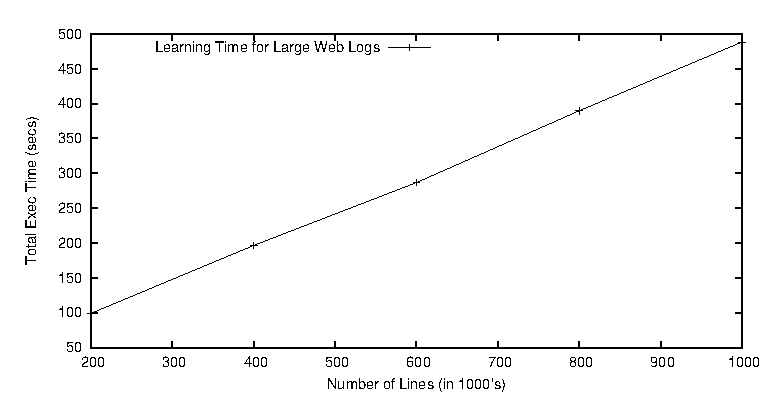
\epsfig{file=scale.eps,width=0.9\columnwidth}
\caption{Scaling of increment algorithm}
\label{fig:scale}
\end{center}
\vskip -2ex
\end{figure}

The second experiment measures the execution time of learning
descriptions for a series of web server logs ranging in size from 200k
to one million lines.  This data source is private to AT\&T, so we ran the experiments on
an AT\&T internal server which runs GNU/Linux and has a 1.60GHz Intel Xeon CPU with 8GB
of memory.
\figref{fig:scale} suggests the incremental algorithm scales linearly
with the number of lines. In particular, the algorithm
learns a description for a million-line web log in under 10
minutes. The inferred description yields a parser that correctly
parses all lines in the log.

% - parse metric
% - initial learn size and chunk size - these can affect results
% - update chunk by chunk 
% - optimizations/heuristics
%   due to performance concerns:
%   - memoization
%   - the clean function (to reduce the number of parses)
%   - control of aggregate size
%   - parses cut-off: kill a parse if it has more than n consecutive failures in a struct
%   due to quality of description concerns (and also performance)
%   - deterministic unions
%   - longest match in arrays
%   - merge adjacent const strings (only punctuation and white spaces)
%   - error recovery
%
%- Experiments
%	1) comparison with old LearnPADS on several large datasets (ai.3000, asl.log, apache.txt, access\_log, error\_log, interface.loop)
%	   compare exec time and type complexity. For increment, use
%	   initial learn chunk of 100 and incremental error chunks of 100
%	2) use ai format, do a table with 1000 5000 10000,...,1M miles
%	   using orig learning system and the new system with various optimization turned on and off.
%

